\documentclass[12pt]{report}
\usepackage[utf8]{inputenc}
\usepackage[main=russian,english]{babel}
\usepackage[left=20mm, top=15mm, right=20mm, bottom=10mm, nohead, nofoot]{geometry}

\usepackage{graphicx}
\usepackage{caption}
\usepackage{wrapfig}
\usepackage{multicol}
\usepackage{lipsum}
\usepackage{mwe}
\usepackage{enumerate}

%\usepackage{listings}
%\lstloadlanguages{java}


% -----------------------------------
%
% !!! Сделать нормальное содержание и ссылки !!!
%
% -----------------------------------

% \def \var {value}
\newcommand{\ReportTheme}{Практика}
\newcommand{\ReportAuthor}{Данилевич Леонид, Лельчук Александр, 2022А класс}

\title{\bf \ReportTheme}
\author{\it \ReportAuthor}
\date{\today}

% 1. Титульный лист. (Одинаковая по форме. Взять в нетскуле)
% 2. Аннотация. (Около абзаца. Кратко, какая поставлена задача, какой результат получен. Делается в последний момент)
% 3. Оглавление.
% 4. Введение. (Где родилась задача. Ваша задача - подспорье в решении какой-то более глобальной. Зачем это всё нужно = Обоснование работы)
% 5. Постановка задачи. Сформулировать задачу так, чтобы можно было её решить математически/померить экспериментально/и т д.
% 6. Методика разрешения задачи. Как решается задача: математически/экспериментально/программно и т д. Подробности. С помощью каких механизмов.
% 7. Результаты. Что вы померили/насчитали/
% 8. Анализ результатов. Что означают результаты. Совпадают ли с предсказаниями. Что следует из результатов.
% 9. Список литературы. На что вы опирались.
% 10. Благодарности. С кем вы работали, кто вас консультировал, кто помогал и т п.

%\usepackage{mathptmx}

\begin{document}
   % \maketitle
   % титульный лист

    \begin{center}
    \large { {\bf Лицей «Физико-техническая школа»  Санкт-Петербургского Академического университета   } } 
    
    \vspace*{6\baselineskip}
    
    \vfill
    \large { {\bf Курсовая работа (отчет по практике) } } 
    
    \vspace*{6\baselineskip}
    
    Создание программы, генерирующей кроссворды из регулярных выражений \\
    \vspace*{3\baselineskip}
    
    \end{center}        
    \begin{flushright}
        Работу выполнили: \\
        Данилевич Леонид (2022А) \\
        Лельчук Александр (2022А) \\
        Научный руководитель: \\
        Дворкин Михаил Эдуардович \\
        Место прохождения практики: \\
        Лицей <<ФТШ>>
    \end{flushright}
    \vspace*{5\baselineskip}
    \begin{center}
        Санкт-Петербург, 2021
    \end{center}        
%----------------------------------------------------------------------------------------------------------
    \newpage % Аннотация
    \chapter*{Аннотация}
    Мы создали программу, генерирующую кроссворды, в которых строки и столбцы описываются регулярными выражениями. В регулярных выражениях используются различные человекочитаемые паттерны (например: палиндромы, прогрессии, словарные ключи, повторы и так далее).
     
    Полученный кроссворд имеет единственное решение, которое может быть получено последовательным сужением круга возможных вариантов - таким образом, для отгадывания кроссворда не требуется подставлять различные буквы, после чего проверять корректность полученного предположением кроссворда.

    Также программа может решить произвольный аналогичный кроссворд (поддерживается ограниченный набор конструкций, составляющих регулярные выражения).

    
%----------------------------------------------------------------------------------------------------------
    \newpage % Оглавление
\renewcommand*\contentsname{Кроссворды из регулярных выражений }
\tableofcontents
%----------------------------------------------------------------------------------------------------------
    \newpage % Введение
\chapter{Введение}
Регулярные выражения — формальный язык поиска подстрок в тексте и манипуляций с ними. Например, регулярному выражению «.*amp(le)?» соответствуют строки «Sample», «example», «lamp» и некоторые другие. С помощью регулярных выражений можно достаточно легко искать в тексте подстроки определённого формата и заменять их на соответствующие им другие подстроки. В 2013 году, как задание конкурса «MIT Mystery Hunt», был создан кроссворд из регулярных выражений (рис. \ref{pic:MITHex}). Мы решили написать приложение, автоматически генерирующее подобные кроссворды, а также позволяющее их решать. Мы считаем, что такое приложение будет полезно многим людям, изучающим регулярные выражения, а для уже знакомых с ними оно будет просто интересно.
 \begin{figure*}[ht!]
 \centering
    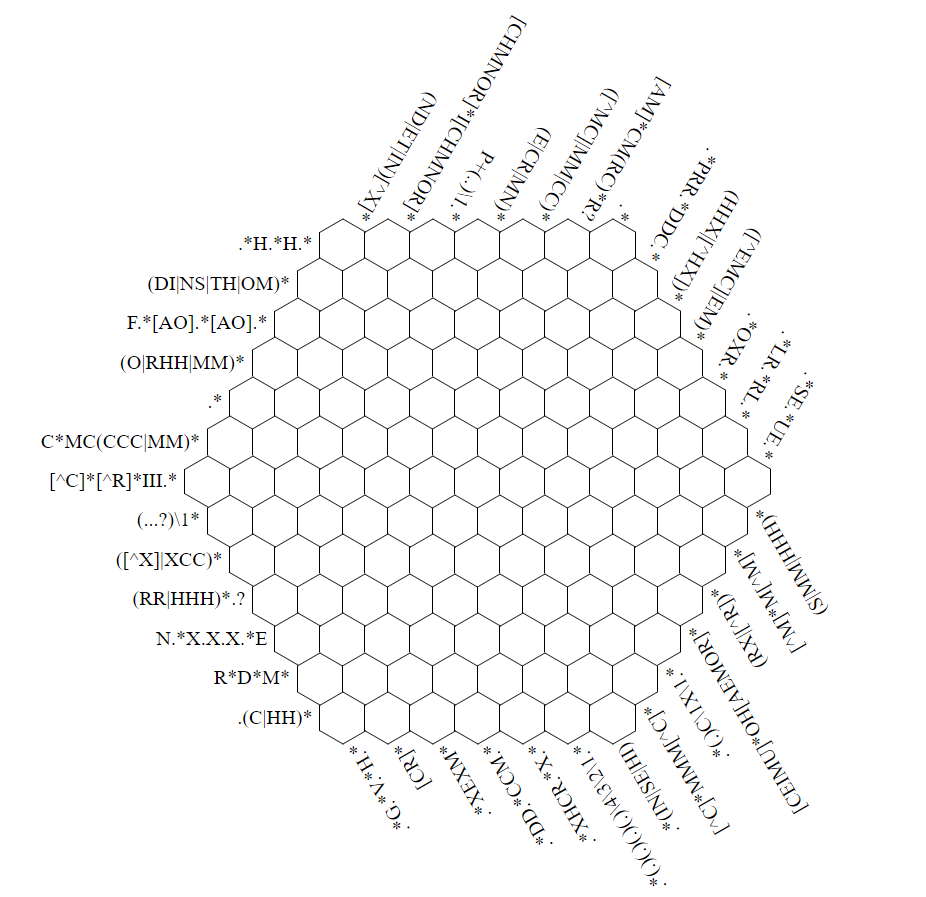
\includegraphics[width=.7\textwidth]{MITHexagon.png}
    \caption{\label{pic:MITHex}Кроссворд с «MIT Mystery Hunt» 2013 года}
\end{figure*}

%----------------------------------------------------------------------------------------------------------
    \newpage % Постановка задачи
   \chapter{Постановка задачи}
   
   Создать приложение на базе Android, функционалом которого является генерация, отображение и поддержка решения пользователем красивых кроссвордов из регулярных выражений.
   
   Кроссворд из регулярных выражений -- клеточная сетка правильной формы (прямоугольник, шестиугольник и т. д.). Решением кроссворда называется такое сопоставление символа каждой клетке, что линии, образованные этими символами (например, в прямоугольнике это столбцы и строчки) формируют буквенные строчки, закодированные соответственными регулярными выражениями.
   
   Мы называем кроссворд из регулярных выражений красивым, если он имеет единственное решение; в нём регулярные выражения, использующиеся для кодирования линий символов, разнообразны (используется большое количество конструкций: символьные классы, группы, перечисления, квантификаторы, обратные ссылки и т. д.); в полученных линиях символов должны наблюдаться паттерны, которые легко воспринимаются человеком.


%----------------------------------------------------------------------------------------------------------
    \newpage % Методика решения задачи
\chapter{Методика решения задачи}

Так как задача состоит в написании программы, то решается программно. Задача дробится на части: 
\section{Программное решение кроссворда}
Собственно, решение уже имеющегося кроссворда. Понадобится для оценки сложности кроссворда и удостоверения единственности решения.

\subsection{Разбор регулярных выражений} Для решения произвольного кроссворда необходимо разобрать («распарсить») регулярные выражения, кодирующие его строчки. Для этого написана рекурсивная функция с запоминанием ответа (техника «мемоизации» динамического программирования), которая для заданного регулярного выражения и требуемой длины строчки находит в компактном виде всевозможные строчки, подходящие под данное выражение. Компактный вид обусловлен тем, что строчки состоят не из символов, а из битовых масок, где из любой маски можно выбрать любой символ и получить корректную строчку. Обратные ссылки в регулярных выражениях обрабатываются следующей техникой: два символа, запрашиваемые быть одинаковыми, соответствуют одному и тому же битовому объекту-маске.

\subsection{Отгадывание букв} После разбора регулярных выражений кроссворд решается методом инкрементальных улучшений. Изначально каждой букве сопоставлена битовая маска, соответствующая всем символам алфавита. Алгоритм рассматривает все ещё не разгаданные буквы по порядку, сужая для каждой множество возможных значений. Существует вероятность встретить кроссворд, имеющий решение, но нерешаемый данной техникой. Однако для его разгадывания человеку потребуется долгий и утомительный перебор. Создание таких кроссвордов не входит в нашу задачу. В случае полного разгадывания кроссворда можно утверждать, что его решение существует и единственно.


\section{Генерация буквенного заполнения кроссворда} 
Первым шагом для генерации произвольного кроссворда является генерация <<буквенного заполнения>> кроссворда, а именно, нахождение поля, которое получит пользователь, правильно разгадавший кроссворд.

\subsection{Оценка стоимости заполнения кроссворда}
Для красоты кроссворда необходимо образование строк, подходящих под различные регулярные выражения. Максимизируется красота заполнения — субъективное свойство, включающее в себя регулярность кроссворда. Именно, максимизируется количество и длина входящих в кроссворд подстрок, являющихся шаблонами следующих типов: палиндром (строка, читающаяся одинаково слева направо и справа налево); повтор (строка, состоящая из одинаковой части, повторённой несколько раз); прогрессия (строка, в которой на нечётных (в 1-индексации) местах стоят одинаковые буквы, а на чётных - разные; словарный ключ - существующее английское слово.

\subsection{Имитация отжига} Для генерации случайного поля, максимизирующего потенциальную стоимость кроссворда, а именно, разнообразие типов регулярных выражений, разгадка необходимой степени сложности, и субъективная оценка красоты, применён метод имитации отжига (<<simulated annealing>>). Каждая итерация отжига заменяет одну букву на изначально равномерно случайно сгенерированном поле, после чего в некотором случае изменение принимается, поле обновляется.


\section{Генерация регулярных выражений} 
Вторым шагом является <<восстановление>> регулярных выражений, описывающих линии - строки и стобцы - кроссворда. Кроссворд должен иметь единственное решение, но не быть очевидным.

\subsection{Оценка стоимости регулярных выражений}
Для оценки стоимости анализируются регулярные выражения в строковом представлении, максимизируется разнообразие паттернов. % Я вообще не знаю, что там делается, напишешь подробнее?)

\subsection{Имитация отжига}
Здесь  также используется метод имитации отжига. Начальные регулярные выражения побуквенно (следовательно, однозначно) задают соответствующие линии кроссворда. На каждой итерации метода имитации отжига регулярное выражение, соответствующее случайной линии кроссворда изменяется. После этого в случае улучшения цены кроссворда (при условии, что кроссворд по-прежнему решается единственным образом) изменение принимается.


\section{Оценка сложности, проверка единственности решения} 
Оценка сложности и проверка единственности решения осуществляется путём программного решения.

Для решения кроссворда в случайном порядке выбираются клетки, буква в которых ещё не определена однозначно, после чего сужается круг возможных значений. Пока неясно, что за буква в ней стоит, одна и та же клетка может быть выбрана сколь угодно много раз. Сложность кроссворда считается как усреднённое количество клеток, которые надо рассмотреть, чтобы полностью решить кроссворд. Очевидно, минимальная сложность равна суммарному количеству всех клеток в кроссворде, но сложность нетривиального кроссворда всегда больше.
   

%----------------------------------------------------------------------------------------------------------
    \newpage % Результаты
    
\chapter{Результаты}
\section{Программное решение кроссворда}
Получившаяся программа успешно разгадывает кроссворды и составляет собственные. При вводе регулярных выражений из кроссворда, упоминавшегося во введении (рис. \ref{pic:MITHex}), программа выдаёт следующее решение (рис. \ref{pic:MITSolution})
\begin{figure*}[ht!]
 \centering
    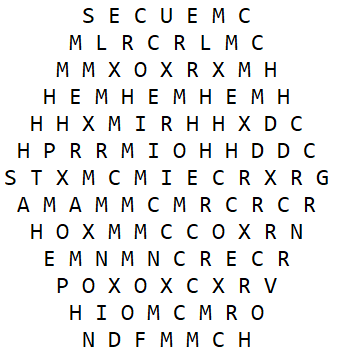
\includegraphics[scale=1.0]{HexagonalOutput1.PNG}
    \caption{\label{pic:MITSolution}Решение кроссворда (рис. \ref{pic:MITHex})}
\end{figure*}
\section{Генерация буквенного заполнения кроссворда}
Алгоритм получилось написать. Результатом является довольно хорошо удовлетворяющие условиям кроссворды (рис. \ref{pic:GenCross}):
\begin{figure*}[p!]
 \centering
    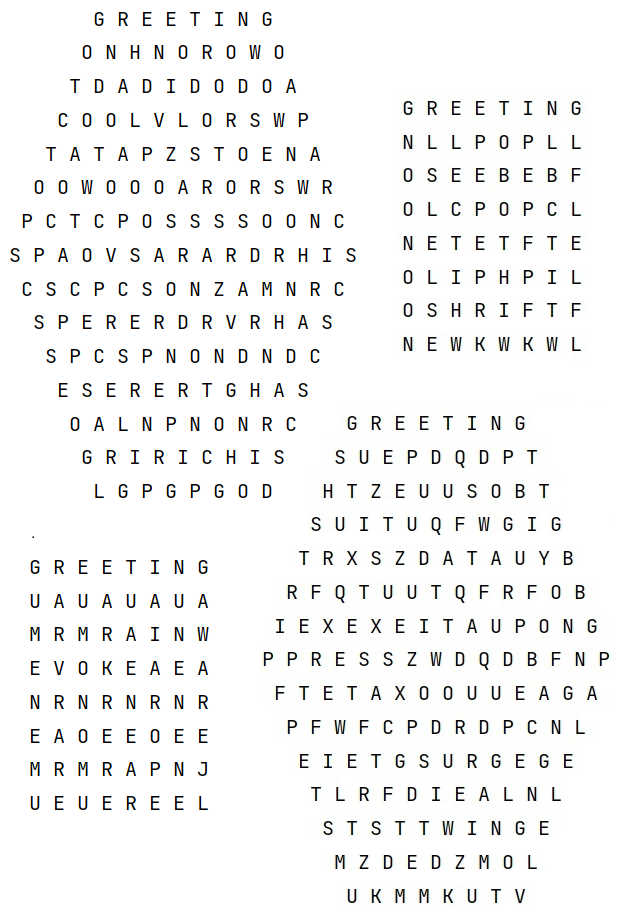
\includegraphics[scale=1.0]{generated8.png}
    \caption{\label{pic:GenCross}Сгенерированные кроссворды}
\end{figure*}
Рассмотрим подробнее результат работы отжига. Выделим некоторые существенные паттерны в одном из кроссвордов (рис. \ref{pic:Patterns})
\begin{figure*}[p!]
 \centering
    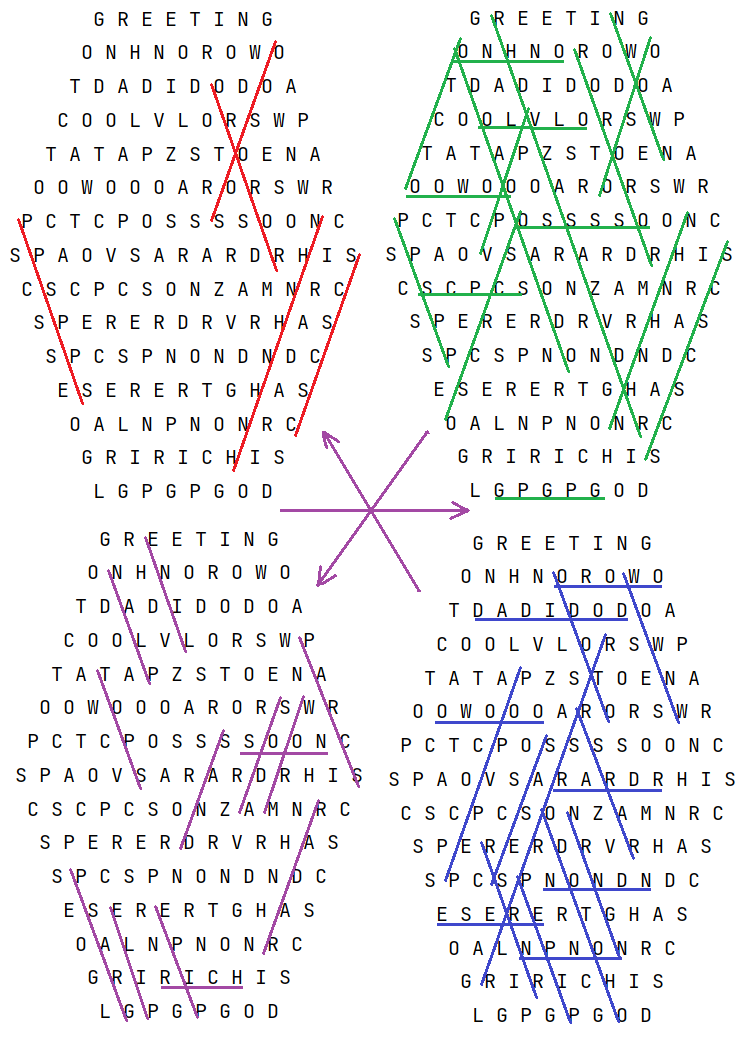
\includegraphics[scale=0.9]{patterns.png}
    \caption{\label{pic:Patterns}Слева направо, сверху вниз: повторы, палиндромы, слова, прогрессии}
\end{figure*}
\section{Генерация регулярных выражений} Регулярные выражения также получилось сгенерировать. На картинке (рис. \ref{pic:CrossWithRegexps}) изображён кроссворд с описывающими строки регулярными выражениями, полученный в результате работы программы.
\begin{figure*}[p!]
 \centering
    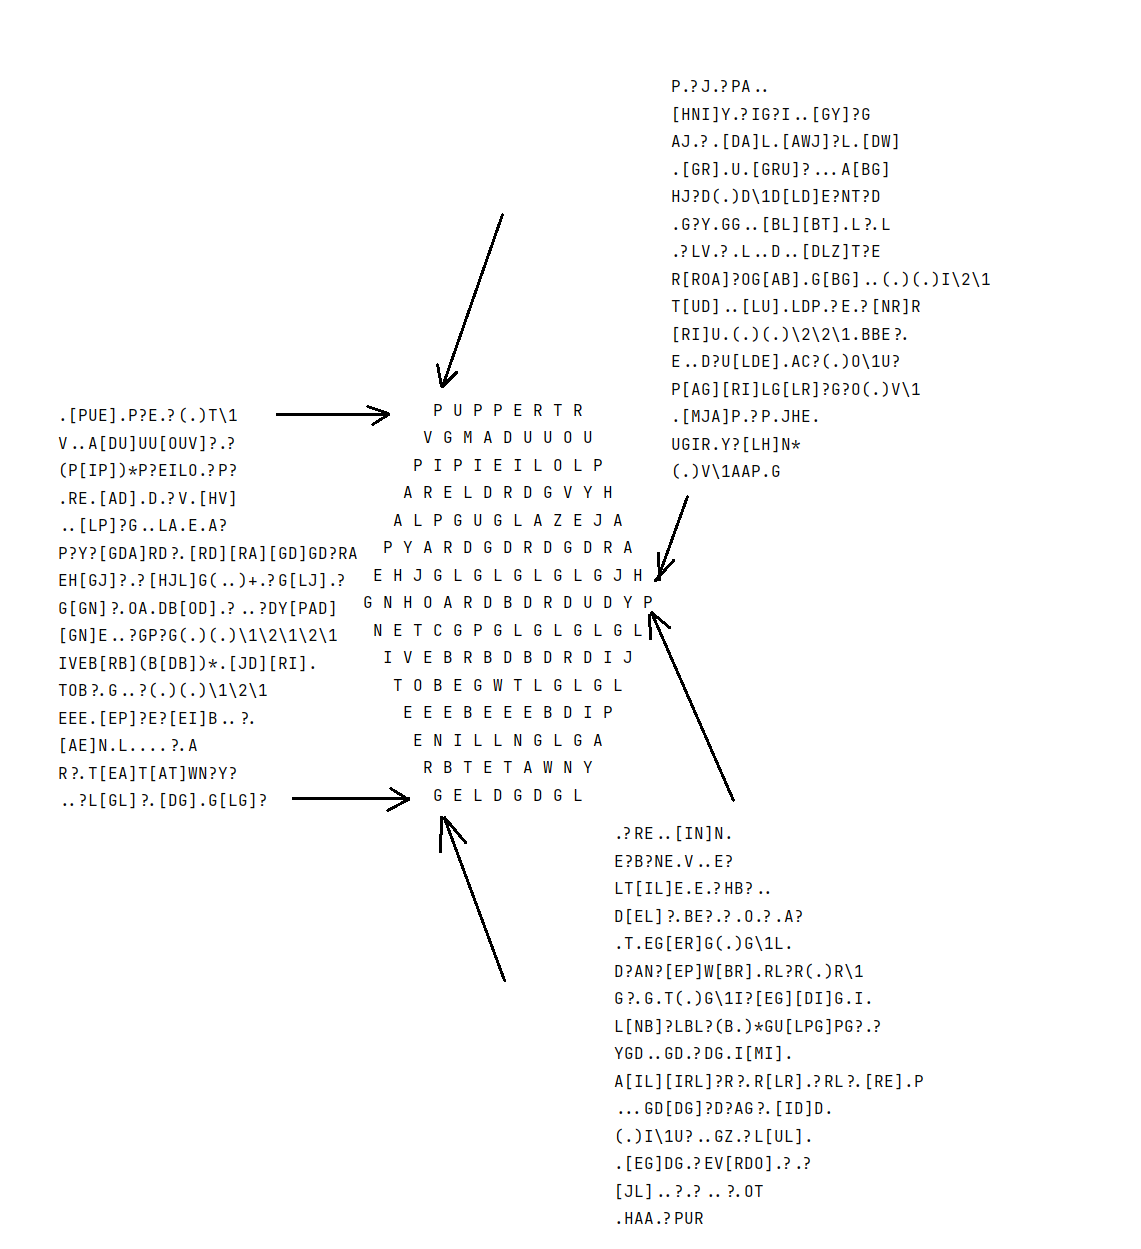
\includegraphics[scale=0.8]{generated9.png}
    \caption{\label{pic:CrossWithRegexps} Кроссворд и регулярные выражения}
\end{figure*}

\section{Оценка сложности, проверка единственности решения} Решение кроссворда заодно проверяет и единственность данного решения. Реализовано, как и написано в методике. Оказалось, что в текущих условиях даже наивная тактика перебора случайных клеток даёт очень неплохие результаты. Так, усреднённое количество клеток, которые нужно выбрать по 10 запускам, чтобы полностью решить приведённый на рисунке (рис. \ref{pic:CrossWithRegexps}) кроссворд из 169 клеток в среднем равно 205. Для сравнения, кроссворд MIT (рис. \ref{pic:MITHex}) решается за 320 итераций, что намного лучше.

%----------------------------------------------------------------------------------------------------------
    \newpage % Анализ рез-ов    
\chapter{Анализ результатов}
Написать программу под Android не удалось. Основная логика программы, а именно, решение и генерация кроссвордов написаны. Она подлежит доработке, так как получившиеся кроссворды решаются слишком быстро.

    
%----------------------------------------------------------------------------------------------------------
%    \newpage % Список литры (у нас пуст в общем)

%----------------------------------------------------------------------------------------------------------
    \newpage % Благодарности
\chapter{Благодарности}
Мы благодарим нашего научного руководителя { \bf Дворкина Михаила Эдуардовича } за научное руководство и направление теоретической части нашей работы.
    \\
    \\
    
    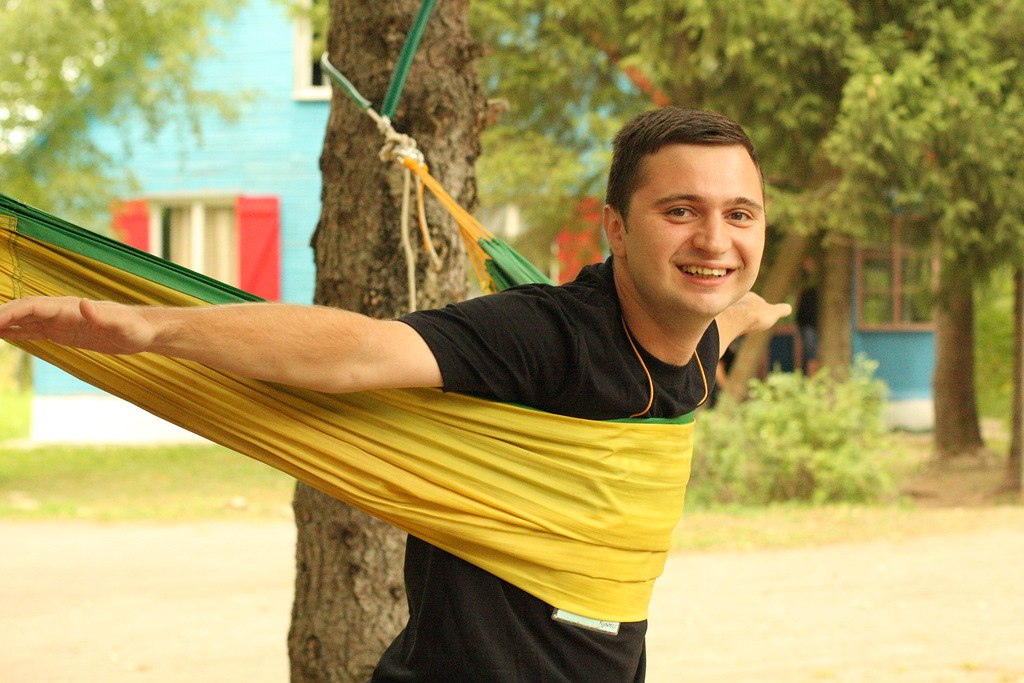
\includegraphics[scale=0.5]{dvorkin2.jpg}\hfill
    

        
\end{document}

